\chapter{Optimization}

The solution presented in Chapter~\ref{chap:solution}, despite
providing correctness guarantees and ease of use, performs poorly in
even trivial test cases. This chapter describes a series of
optimizations made to keep the overhead as low as possible, without
sacrificing correctness.

\section{Example Application}

To perform accurate measurements, a sample banking application was
developed. In this application's domain there is a central Bank with
Customers, which in turn have their accounts. For each account there
is a slot representing the account's balance, and there is a method to
show a customer's balance (by summing the balance of all his
accounts). Every time a transaction is done, a new TransactionRecord
is created, containing a timestamp, the origin and destination
accounts, as well as the amount transfered.

In this scenario, a Business Transaction will be made of several
banking transactions throughout a series of steps. This is the perfect
candidate for a Long Lived Transaction.

With the support presented in previous sections, the programmer simply
writes the application's code as he would without considering Long
Lived Transactions. No changes to the data structures and business
logic are required.

Using this banking domain, a sample application was developed. In this
fictitious scenario, the bank would start with a certain number of
customers (this number was configurable so different parameters could
be measured), create a Long Lived Transaction with a configurable
number of steps. Within each step, new customers and accounts would be
created, money would be shuffled between all the bank's accounts
(creating a new TransactionRecord for each transaction), and the total
balance is calculated. This means that in each step: 1) Every object
is read, 2) Many objects are written, 3) Many objects are created.

\section{Initial Solution Performance}

Figure~\ref{fig:regTime} shows the running time for a varying number
of iterations on the application presented above. As expected, the
running time grows linearly as the number of iterations increases.

When looking at the Long Lived version (where every iteration is a
step of a large Long Lived Transaction), performance quickly degrades
as the number of iterations grows {\it O(n3)}. This is due to the fact
that many boxes must be read in order to look up write set entries.

\begin{figure}
\centering
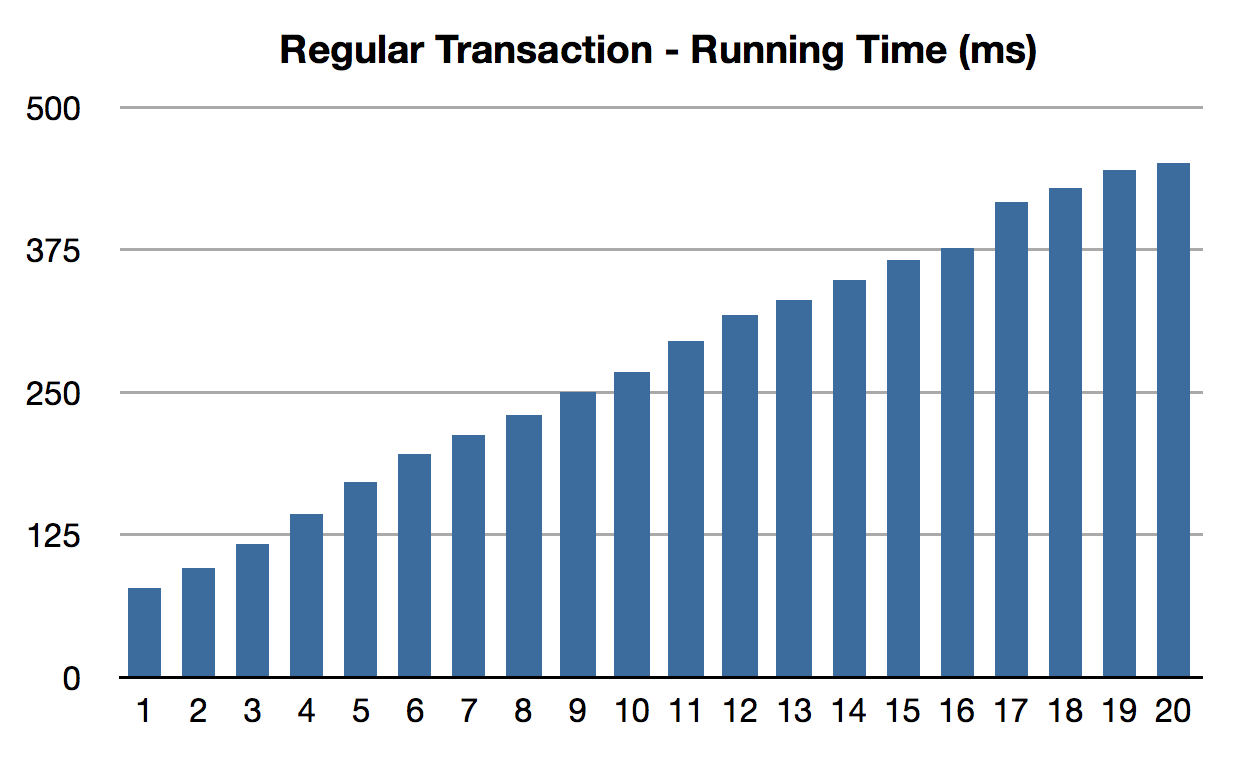
\includegraphics[width=0.7\linewidth]{reg-time}
\caption{Running time with regular transactions}
\label{fig:regTime}
\end{figure}

\begin{figure}
\centering
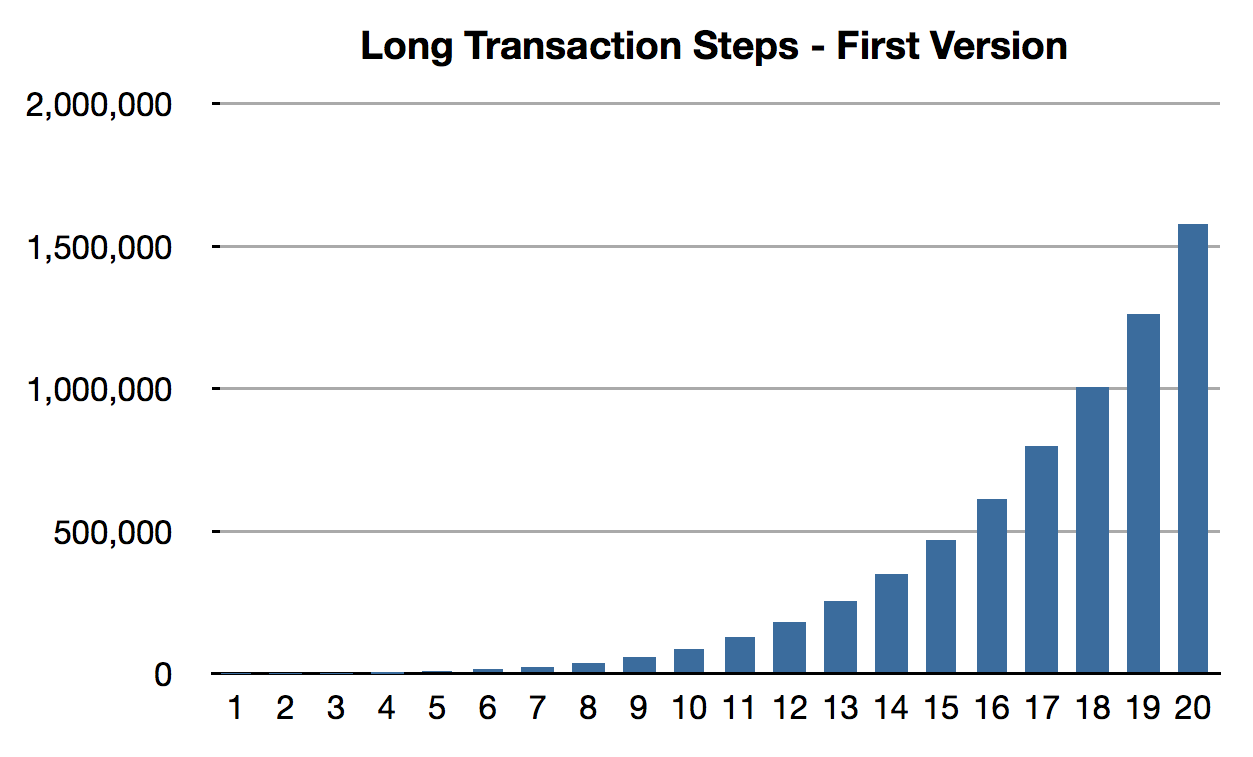
\includegraphics[width=0.7\linewidth]{long-time-v1}
\caption{Running time with Long Lived Transaction steps}
\end{figure}

\begin{figure}
\centering
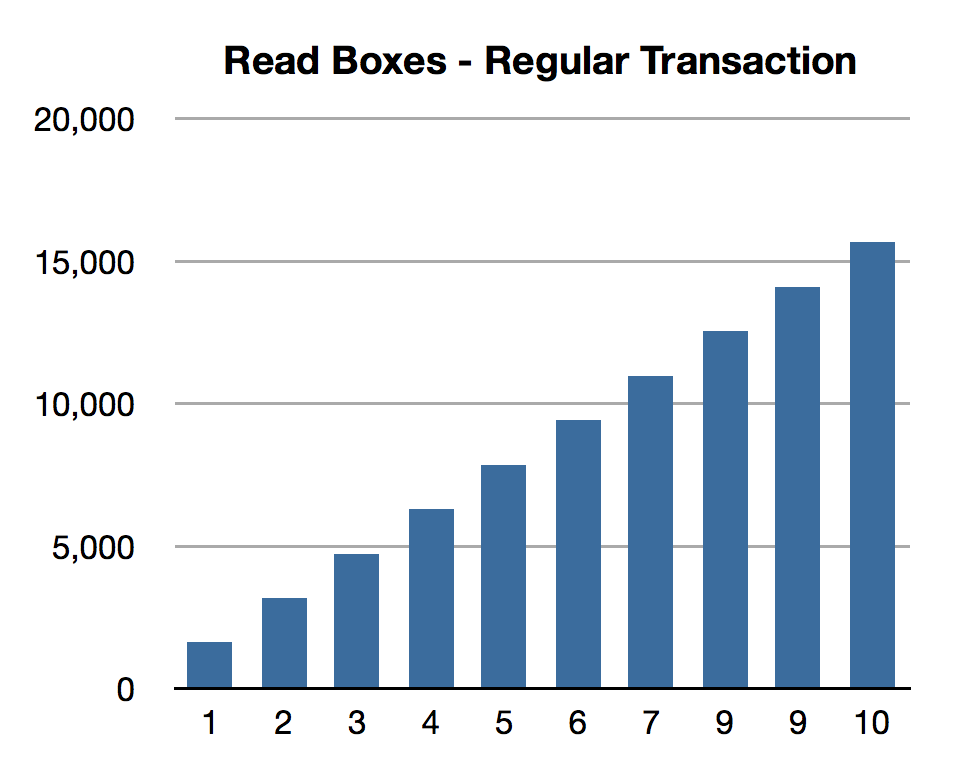
\includegraphics[width=0.6\linewidth]{reg-box}
\caption{Running time with Long Lived Transaction steps}
\end{figure}

\begin{figure}
\centering
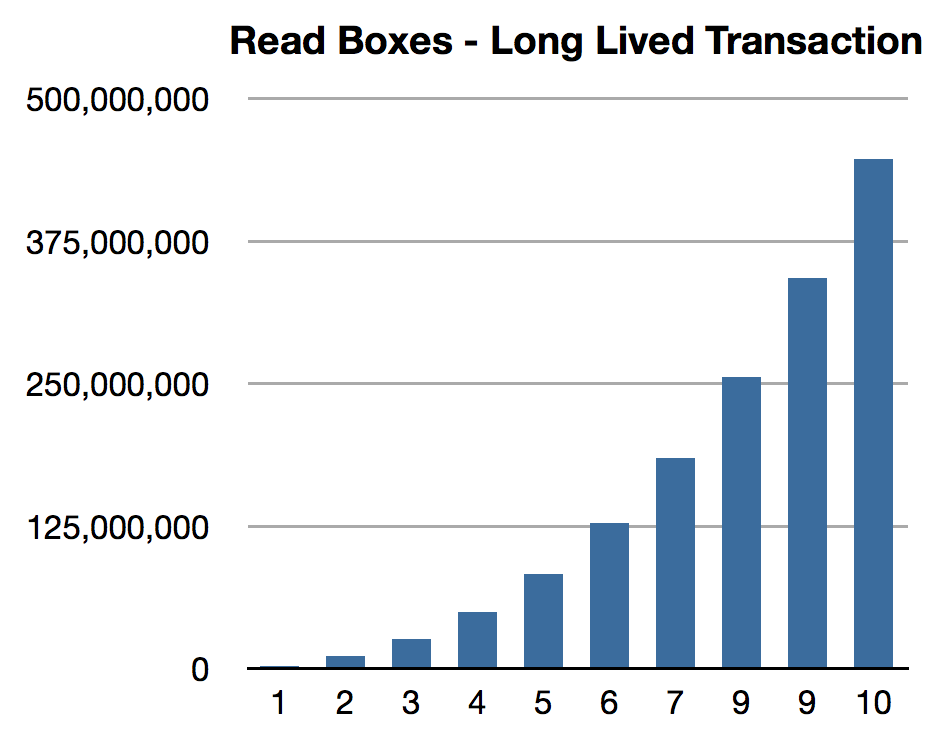
\includegraphics[width=0.6\linewidth]{long-box-v1}
\caption{Running time with Long Lived Transaction steps}
\end{figure}

\section{Read-Set differentiation}

In the implementation described in Chapter \ref{chap:solution}, both
the Write-Set and the Read-Set were represented using {\it LogEntries}.

Recalling Figure \ref{fig:architecture}, {\it LogEntries} store a
reference to the respective DomainObject, the object's slot, and the
slot's value. These objects were used to store elements of both the
Read Set and the Write Set, which proved to be quite expensive, as the
Read Set only cares about which slots were read, completely
ignoring its value.

Carefully looking at the nature of the Read Set, one comes to realise
that it is only necessary to store the pairs [DomainObject, Slot] read
by the transaction (the actual version read is not relevant, as it
will always be coherent with the transaction's version).

As such, the Read Set has been replaced by an immutable
ValueType\footnote{ValueTypes are explained in detail in Chapter
  \ref{chap:ff}}, containing a set of DomainSlotKey's (an immutable,
lightweight object representing the pair [DomainObject, Slot]), stored
directly into the {\it TransactionalContext}.

This optimization greatly reduced the space required by the
Transaction (both in-memory and persistently), as the representation
of the Read-Set became more compact (a single slot in an object vs
several objects).

The commit time for the various steps of the Transaction also
improved, as the lookups/insertions of entries in the Read Set are
done entirely in memory, without the need to traverse (and
potentially reload a large object graph).

\section{Using BPlusTrees to hold LogEntries}

As described in Chapter \ref{chap:ff}, the Fenix Framework uses
BPlusTrees and other collections to implement to-many relations. These
collections are transparently handled by the Framework, and are
implemented using regular Domain Objects (such as Leaf Nodes and Inner
Nodes). It is then desirable to store the correct values of those
objects within the context of a Long Transaction, as changes in
relations are part of our transparent programming model.

This posed a great issue, as it meant that the relation between a {\it
  TransactionalContext} and the {\it LogEntries} is precisely a
one-to-many relation (and thus backed by a BPlusTree). ???

The initial solution to this problem was implementing the one-to-many
relation as a Linked List, as shown in Figure
\ref{fig:linkedList}. This approach proved to be quite inefficient, as
lookups in the Write Set were {\it O(n)} in the number of written
objects, making it impractical, as every {\it getBoxValue} operation
requires traversing the whole list.

\begin{figure}
  \centering
  \begin{tikzpicture}

\begin{class}[text width=5cm]{TransactionalContext}{5,0}
\end{class}

\begin{class}[text width=2cm]{LogEntry}{5,-2}
\end{class}

\begin{class}[text width=2cm]{LogEntry }{10,-2}
\end{class}

\association{TransactionalContext}{}{}{LogEntry}{writeSet}{0..1}
\unidirectionalAssociation{LogEntry}{nextEntry}{}{LogEntry }

\end{tikzpicture}

\caption{}
\label{fig:linkedList}
\end{figure}

To solve this problem, a specialised sub-class of BPlusTree was
developed, which falls outside the scope of the Long Transaction,
allowing the one-to-many relation to be implemented ???

With this, lookup times were now great!

\section{Removing LogEntries}

With the relation between the {\it TransactionalContext} and the {\it
  LogEntries} implemented using a BPlusTree, another issue arisen. 

Despite having great lookup times, the commit of a Long Transactions's
step was greatly affected. Whereas inserting elements in a Linked List
is {\it O(1)}, the insertion in the BPlusTree was still painfully
slow.

This is because the Fenix Framework requires that ValueTypes (such as
the ones used to back the BPlusTree) are immutable combined with the
fact that the BPlusTree provides no API for batch insertion, meaning
that for each of the elements written within a given step, a new
insert was performed, and the backing TreeMaps were duplicated over
and over. <CONTINUE>.

The approach to solve this issue, was to use a solution similar to the
one used for the Read-Set: create an immutable ValueType, containing
the mapping between all written slots and their respective values.

With this change, {\it LogEntries} were completely taken out of the
picture, as the only extra piece of information they provided was the
JSON contents of the slot, which could be embedded directly into the
WriteSet object.

The issue with this approach, is that due to the immutability
requirement, every time a batch of entries was inserted, the whole Map
had to be duplicated, which was rather wasteful both in terms of time
and allocated memory. So, instead of duplicating the whole Map, the
WriteSet is actually a Linked-List of Maps, containing one node per
transaction step. This meant that the performance of lookups is now
{\it O(s*log(n))}, {\it n} being the average size of each step, and
{\it s} the number of steps (in which something is written) of the
transaction.

\section{Fine tuning WriteSet}

